\documentclass[]{article}
\usepackage{lmodern}
\usepackage{amssymb,amsmath}
\usepackage{ifxetex,ifluatex}
\usepackage{fixltx2e} % provides \textsubscript
\ifnum 0\ifxetex 1\fi\ifluatex 1\fi=0 % if pdftex
  \usepackage[T1]{fontenc}
  \usepackage[utf8]{inputenc}
\else % if luatex or xelatex
  \ifxetex
    \usepackage{mathspec}
  \else
    \usepackage{fontspec}
  \fi
  \defaultfontfeatures{Ligatures=TeX,Scale=MatchLowercase}
\fi
% use upquote if available, for straight quotes in verbatim environments
\IfFileExists{upquote.sty}{\usepackage{upquote}}{}
% use microtype if available
\IfFileExists{microtype.sty}{%
\usepackage{microtype}
\UseMicrotypeSet[protrusion]{basicmath} % disable protrusion for tt fonts
}{}
\usepackage[margin=1in]{geometry}
\usepackage{hyperref}
\hypersetup{unicode=true,
            pdftitle={hw7},
            pdfauthor={LuchaoQi},
            pdfborder={0 0 0},
            breaklinks=true}
\urlstyle{same}  % don't use monospace font for urls
\usepackage{color}
\usepackage{fancyvrb}
\newcommand{\VerbBar}{|}
\newcommand{\VERB}{\Verb[commandchars=\\\{\}]}
\DefineVerbatimEnvironment{Highlighting}{Verbatim}{commandchars=\\\{\}}
% Add ',fontsize=\small' for more characters per line
\usepackage{framed}
\definecolor{shadecolor}{RGB}{248,248,248}
\newenvironment{Shaded}{\begin{snugshade}}{\end{snugshade}}
\newcommand{\KeywordTok}[1]{\textcolor[rgb]{0.13,0.29,0.53}{\textbf{#1}}}
\newcommand{\DataTypeTok}[1]{\textcolor[rgb]{0.13,0.29,0.53}{#1}}
\newcommand{\DecValTok}[1]{\textcolor[rgb]{0.00,0.00,0.81}{#1}}
\newcommand{\BaseNTok}[1]{\textcolor[rgb]{0.00,0.00,0.81}{#1}}
\newcommand{\FloatTok}[1]{\textcolor[rgb]{0.00,0.00,0.81}{#1}}
\newcommand{\ConstantTok}[1]{\textcolor[rgb]{0.00,0.00,0.00}{#1}}
\newcommand{\CharTok}[1]{\textcolor[rgb]{0.31,0.60,0.02}{#1}}
\newcommand{\SpecialCharTok}[1]{\textcolor[rgb]{0.00,0.00,0.00}{#1}}
\newcommand{\StringTok}[1]{\textcolor[rgb]{0.31,0.60,0.02}{#1}}
\newcommand{\VerbatimStringTok}[1]{\textcolor[rgb]{0.31,0.60,0.02}{#1}}
\newcommand{\SpecialStringTok}[1]{\textcolor[rgb]{0.31,0.60,0.02}{#1}}
\newcommand{\ImportTok}[1]{#1}
\newcommand{\CommentTok}[1]{\textcolor[rgb]{0.56,0.35,0.01}{\textit{#1}}}
\newcommand{\DocumentationTok}[1]{\textcolor[rgb]{0.56,0.35,0.01}{\textbf{\textit{#1}}}}
\newcommand{\AnnotationTok}[1]{\textcolor[rgb]{0.56,0.35,0.01}{\textbf{\textit{#1}}}}
\newcommand{\CommentVarTok}[1]{\textcolor[rgb]{0.56,0.35,0.01}{\textbf{\textit{#1}}}}
\newcommand{\OtherTok}[1]{\textcolor[rgb]{0.56,0.35,0.01}{#1}}
\newcommand{\FunctionTok}[1]{\textcolor[rgb]{0.00,0.00,0.00}{#1}}
\newcommand{\VariableTok}[1]{\textcolor[rgb]{0.00,0.00,0.00}{#1}}
\newcommand{\ControlFlowTok}[1]{\textcolor[rgb]{0.13,0.29,0.53}{\textbf{#1}}}
\newcommand{\OperatorTok}[1]{\textcolor[rgb]{0.81,0.36,0.00}{\textbf{#1}}}
\newcommand{\BuiltInTok}[1]{#1}
\newcommand{\ExtensionTok}[1]{#1}
\newcommand{\PreprocessorTok}[1]{\textcolor[rgb]{0.56,0.35,0.01}{\textit{#1}}}
\newcommand{\AttributeTok}[1]{\textcolor[rgb]{0.77,0.63,0.00}{#1}}
\newcommand{\RegionMarkerTok}[1]{#1}
\newcommand{\InformationTok}[1]{\textcolor[rgb]{0.56,0.35,0.01}{\textbf{\textit{#1}}}}
\newcommand{\WarningTok}[1]{\textcolor[rgb]{0.56,0.35,0.01}{\textbf{\textit{#1}}}}
\newcommand{\AlertTok}[1]{\textcolor[rgb]{0.94,0.16,0.16}{#1}}
\newcommand{\ErrorTok}[1]{\textcolor[rgb]{0.64,0.00,0.00}{\textbf{#1}}}
\newcommand{\NormalTok}[1]{#1}
\usepackage{longtable,booktabs}
\usepackage{graphicx,grffile}
\makeatletter
\def\maxwidth{\ifdim\Gin@nat@width>\linewidth\linewidth\else\Gin@nat@width\fi}
\def\maxheight{\ifdim\Gin@nat@height>\textheight\textheight\else\Gin@nat@height\fi}
\makeatother
% Scale images if necessary, so that they will not overflow the page
% margins by default, and it is still possible to overwrite the defaults
% using explicit options in \includegraphics[width, height, ...]{}
\setkeys{Gin}{width=\maxwidth,height=\maxheight,keepaspectratio}
\IfFileExists{parskip.sty}{%
\usepackage{parskip}
}{% else
\setlength{\parindent}{0pt}
\setlength{\parskip}{6pt plus 2pt minus 1pt}
}
\setlength{\emergencystretch}{3em}  % prevent overfull lines
\providecommand{\tightlist}{%
  \setlength{\itemsep}{0pt}\setlength{\parskip}{0pt}}
\setcounter{secnumdepth}{0}
% Redefines (sub)paragraphs to behave more like sections
\ifx\paragraph\undefined\else
\let\oldparagraph\paragraph
\renewcommand{\paragraph}[1]{\oldparagraph{#1}\mbox{}}
\fi
\ifx\subparagraph\undefined\else
\let\oldsubparagraph\subparagraph
\renewcommand{\subparagraph}[1]{\oldsubparagraph{#1}\mbox{}}
\fi

%%% Use protect on footnotes to avoid problems with footnotes in titles
\let\rmarkdownfootnote\footnote%
\def\footnote{\protect\rmarkdownfootnote}

%%% Change title format to be more compact
\usepackage{titling}

% Create subtitle command for use in maketitle
\newcommand{\subtitle}[1]{
  \posttitle{
    \begin{center}\large#1\end{center}
    }
}

\setlength{\droptitle}{-2em}

  \title{hw7}
    \pretitle{\vspace{\droptitle}\centering\huge}
  \posttitle{\par}
    \author{LuchaoQi}
    \preauthor{\centering\large\emph}
  \postauthor{\par}
      \predate{\centering\large\emph}
  \postdate{\par}
    \date{December 13, 2018}


\begin{document}
\maketitle

\subsection{Problem 1}\label{problem-1}

\subsubsection{a.}\label{a.}

Using \(\chi^2\) test:

\begin{Shaded}
\begin{Highlighting}[]
\NormalTok{E11=}\DecValTok{250}
\NormalTok{E12=}\DecValTok{250}
\NormalTok{E21=}\DecValTok{250}
\NormalTok{E22=}\DecValTok{250}
\NormalTok{O11=}\DecValTok{218}
\NormalTok{O12=}\DecValTok{278}
\NormalTok{O21=}\DecValTok{227}
\NormalTok{O22=}\DecValTok{277}
\NormalTok{TS =}\StringTok{ }\NormalTok{(O11}\OperatorTok{-}\NormalTok{E11)}\OperatorTok{^}\DecValTok{2}\OperatorTok{/}\NormalTok{E11}\OperatorTok{+}\NormalTok{(O12}\OperatorTok{-}\NormalTok{E12)}\OperatorTok{^}\DecValTok{2}\OperatorTok{/}\NormalTok{E12}\OperatorTok{+}\NormalTok{(O21}\OperatorTok{-}\NormalTok{E21)}\OperatorTok{^}\DecValTok{2}\OperatorTok{/}\NormalTok{E21}\OperatorTok{+}\NormalTok{(O22}\OperatorTok{-}\NormalTok{E22)}\OperatorTok{^}\DecValTok{2}\OperatorTok{/}\NormalTok{E22}
\KeywordTok{pchisq}\NormalTok{(TS,}\DecValTok{1}\NormalTok{,}\DataTypeTok{lower.tail =} \OtherTok{FALSE}\NormalTok{)}
\end{Highlighting}
\end{Shaded}

\begin{verbatim}
## [1] 0.0004617806
\end{verbatim}

So we reject the null that they are independently and identically
distributed with males and females equally likely.

\subsubsection{b.}\label{b.}

\begin{Shaded}
\begin{Highlighting}[]
\NormalTok{data=}\KeywordTok{matrix}\NormalTok{(}\KeywordTok{c}\NormalTok{(}\DecValTok{218}\NormalTok{,}\DecValTok{278}\NormalTok{,}\DecValTok{227}\NormalTok{,}\DecValTok{277}\NormalTok{),}\DecValTok{2}\NormalTok{)}
\KeywordTok{chisq.test}\NormalTok{(data,}\DataTypeTok{correct =} \OtherTok{FALSE}\NormalTok{)}
\end{Highlighting}
\end{Shaded}

\begin{verbatim}
## 
##  Pearson's Chi-squared test
## 
## data:  data
## X-squared = 0.11983, df = 1, p-value = 0.7292
\end{verbatim}

p-value\textgreater{}0.05, we fail to reject the null that they are
independent.

\subsection{Problem 2}\label{problem-2}

Same as Problem 1 in homework 6:\\
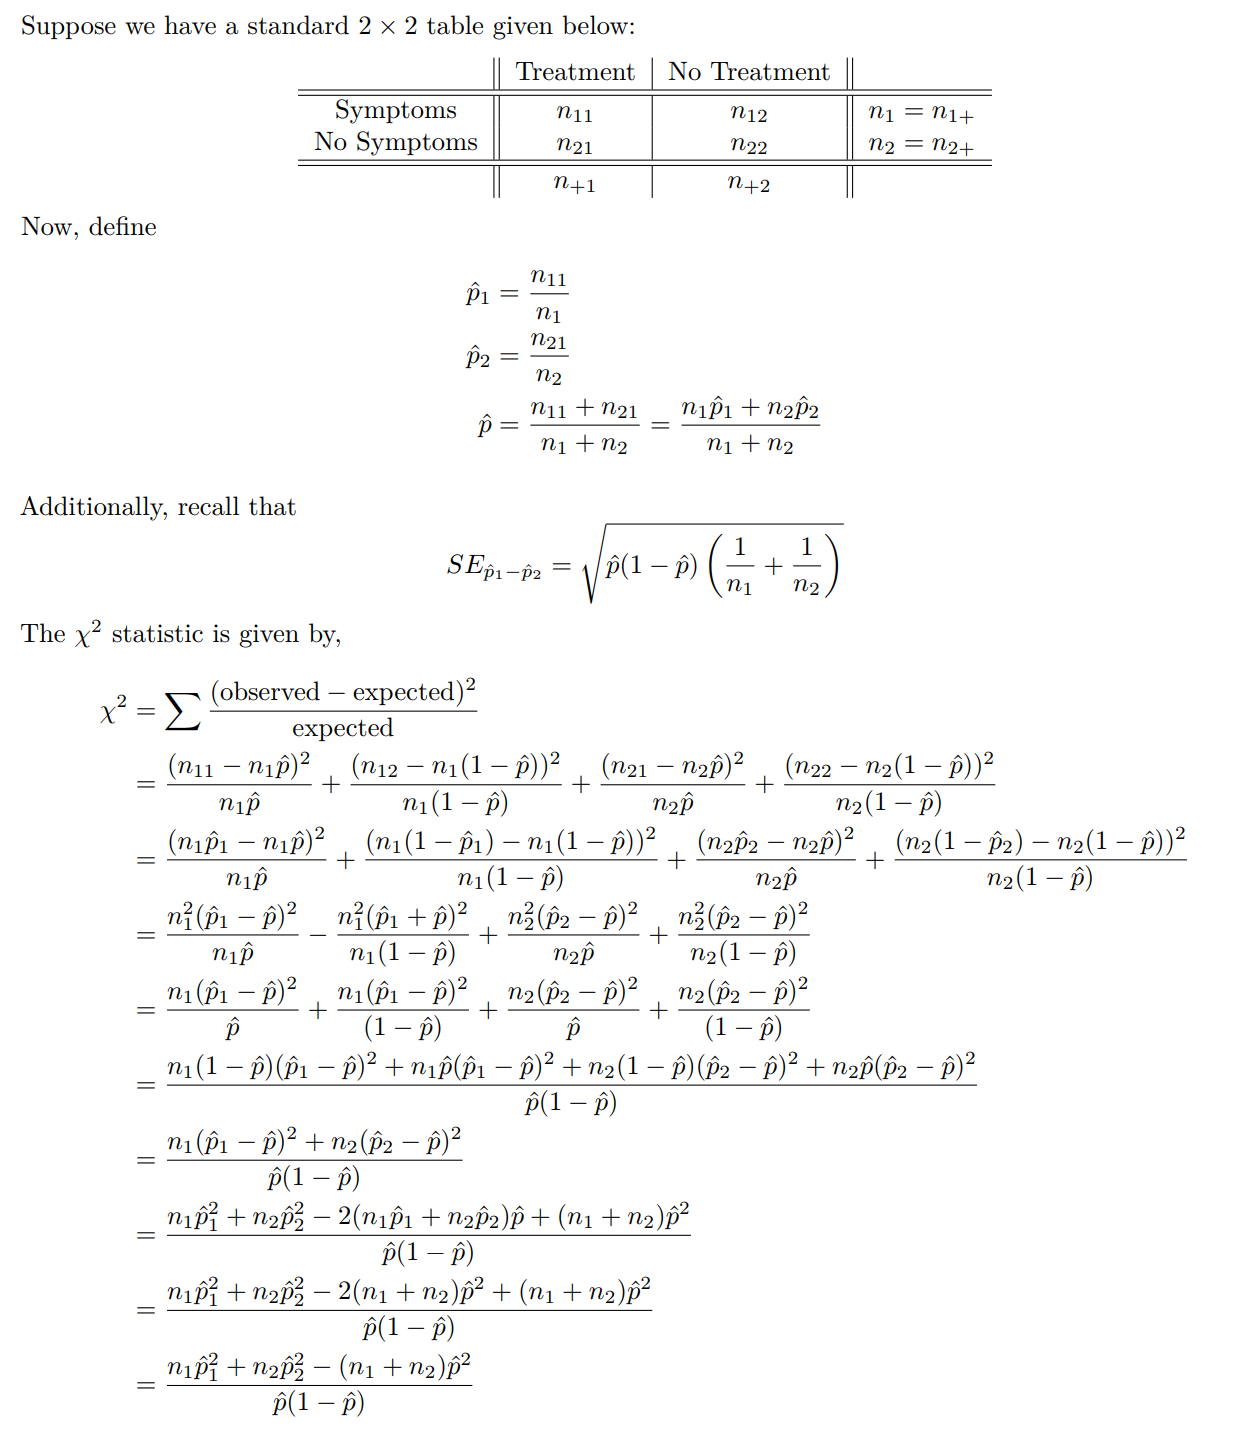
\includegraphics{C:/Users/lcqi/OneDrive/Desktop/3.png}\\
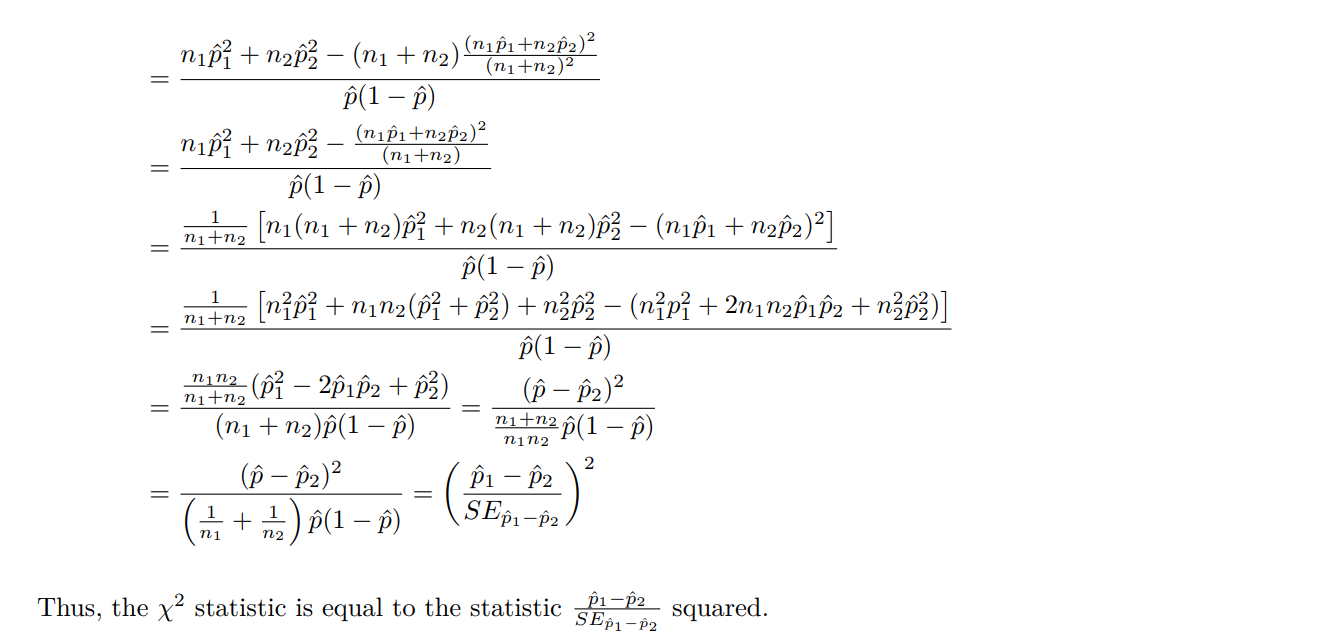
\includegraphics{C:/Users/lcqi/OneDrive/Desktop/4.png}

\subsection{Problem 3}\label{problem-3}

\subsubsection{a.}\label{a.-1}

\(H_0: p1=p2\)\\
\(H_A: p1\neq p2\)\\
There are cases:

Table1 =

\begin{longtable}[]{@{}ll@{}}
\toprule
0 & 15\tabularnewline
\midrule
\endhead
6 & 13\tabularnewline
\bottomrule
\end{longtable}

Table2 =

\begin{longtable}[]{@{}ll@{}}
\toprule
1 & 14\tabularnewline
\midrule
\endhead
5 & 14\tabularnewline
\bottomrule
\end{longtable}

Table3 =

\begin{longtable}[]{@{}ll@{}}
\toprule
2 & 13\tabularnewline
\midrule
\endhead
4 & 15\tabularnewline
\bottomrule
\end{longtable}

Table4 =

\begin{longtable}[]{@{}ll@{}}
\toprule
3 & 12\tabularnewline
\midrule
\endhead
3 & 16\tabularnewline
\bottomrule
\end{longtable}

Table5 =

\begin{longtable}[]{@{}ll@{}}
\toprule
4 & 11\tabularnewline
\midrule
\endhead
2 & 17\tabularnewline
\bottomrule
\end{longtable}

Table6 =

\begin{longtable}[]{@{}ll@{}}
\toprule
4 & 11\tabularnewline
\midrule
\endhead
2 & 17\tabularnewline
\bottomrule
\end{longtable}

Table7 =

\begin{longtable}[]{@{}ll@{}}
\toprule
6 & 9\tabularnewline
\midrule
\endhead
0 & 19\tabularnewline
\bottomrule
\end{longtable}

\begin{Shaded}
\begin{Highlighting}[]
\KeywordTok{choose}\NormalTok{(}\DecValTok{15}\NormalTok{,}\DecValTok{0}\NormalTok{)}\OperatorTok{*}\KeywordTok{choose}\NormalTok{(}\DecValTok{19}\NormalTok{,}\DecValTok{6}\NormalTok{)}\OperatorTok{/}\KeywordTok{choose}\NormalTok{(}\DecValTok{34}\NormalTok{,}\DecValTok{6}\NormalTok{)}\OperatorTok{+}\KeywordTok{choose}\NormalTok{(}\DecValTok{15}\NormalTok{,}\DecValTok{1}\NormalTok{)}\OperatorTok{*}\KeywordTok{choose}\NormalTok{(}\DecValTok{19}\NormalTok{,}\DecValTok{5}\NormalTok{)}\OperatorTok{/}\KeywordTok{choose}\NormalTok{(}\DecValTok{34}\NormalTok{,}\DecValTok{6}\NormalTok{)}\OperatorTok{+}
\StringTok{  }\KeywordTok{choose}\NormalTok{(}\DecValTok{15}\NormalTok{,}\DecValTok{2}\NormalTok{)}\OperatorTok{*}\KeywordTok{choose}\NormalTok{(}\DecValTok{19}\NormalTok{,}\DecValTok{4}\NormalTok{)}\OperatorTok{/}\KeywordTok{choose}\NormalTok{(}\DecValTok{34}\NormalTok{,}\DecValTok{6}\NormalTok{)}\OperatorTok{+}\KeywordTok{choose}\NormalTok{(}\DecValTok{15}\NormalTok{,}\DecValTok{4}\NormalTok{)}\OperatorTok{*}\KeywordTok{choose}\NormalTok{(}\DecValTok{19}\NormalTok{,}\DecValTok{2}\NormalTok{)}\OperatorTok{/}\KeywordTok{choose}\NormalTok{(}\DecValTok{34}\NormalTok{,}\DecValTok{6}\NormalTok{)}\OperatorTok{+}
\StringTok{  }\KeywordTok{choose}\NormalTok{(}\DecValTok{15}\NormalTok{,}\DecValTok{5}\NormalTok{)}\OperatorTok{*}\KeywordTok{choose}\NormalTok{(}\DecValTok{19}\NormalTok{,}\DecValTok{1}\NormalTok{)}\OperatorTok{/}\KeywordTok{choose}\NormalTok{(}\DecValTok{34}\NormalTok{,}\DecValTok{6}\NormalTok{)}\OperatorTok{+}\KeywordTok{choose}\NormalTok{(}\DecValTok{15}\NormalTok{,}\DecValTok{6}\NormalTok{)}\OperatorTok{*}\KeywordTok{choose}\NormalTok{(}\DecValTok{19}\NormalTok{,}\DecValTok{0}\NormalTok{)}\OperatorTok{/}\KeywordTok{choose}\NormalTok{(}\DecValTok{34}\NormalTok{,}\DecValTok{6}\NormalTok{)}
\end{Highlighting}
\end{Shaded}

\begin{verbatim}
## [1] 0.6721736
\end{verbatim}

p-value = 0.6721736

\begin{Shaded}
\begin{Highlighting}[]
\NormalTok{data=}\KeywordTok{matrix}\NormalTok{(}\KeywordTok{c}\NormalTok{(}\DecValTok{2}\NormalTok{,}\DecValTok{13}\NormalTok{,}\DecValTok{4}\NormalTok{,}\DecValTok{15}\NormalTok{),}\DecValTok{2}\NormalTok{)}
\KeywordTok{fisher.test}\NormalTok{(data,}\DataTypeTok{alternative =} \StringTok{"two.sided"}\NormalTok{)}
\end{Highlighting}
\end{Shaded}

\begin{verbatim}
## 
##  Fisher's Exact Test for Count Data
## 
## data:  data
## p-value = 0.6722
## alternative hypothesis: true odds ratio is not equal to 1
## 95 percent confidence interval:
##  0.04590206 4.89390008
## sample estimates:
## odds ratio 
##   0.586089
\end{verbatim}

\subsubsection{b.}\label{b.-1}

For normal statistics: using score test

\begin{Shaded}
\begin{Highlighting}[]
\NormalTok{p1=}\DecValTok{2}\OperatorTok{/}\DecValTok{15}
\NormalTok{p2=}\DecValTok{4}\OperatorTok{/}\DecValTok{19}
\NormalTok{p=}\DecValTok{6}\OperatorTok{/}\DecValTok{34}
\NormalTok{TS =}\StringTok{ }\NormalTok{(p1}\OperatorTok{-}\NormalTok{p2)}\OperatorTok{/}\KeywordTok{sqrt}\NormalTok{(p}\OperatorTok{*}\NormalTok{(}\DecValTok{1}\OperatorTok{-}\NormalTok{p)}\OperatorTok{*}\NormalTok{(}\DecValTok{1}\OperatorTok{/}\DecValTok{15}\OperatorTok{+}\DecValTok{1}\OperatorTok{/}\DecValTok{19}\NormalTok{))}
\KeywordTok{pnorm}\NormalTok{(TS)}\OperatorTok{*}\DecValTok{2}
\end{Highlighting}
\end{Shaded}

\begin{verbatim}
## [1] 0.5577055
\end{verbatim}

For \(\chi^2\) statistics:

\begin{Shaded}
\begin{Highlighting}[]
\NormalTok{e11=}\DecValTok{6}\OperatorTok{/}\DecValTok{34}\OperatorTok{*}\DecValTok{15}
\NormalTok{e12=}\DecValTok{28}\OperatorTok{/}\DecValTok{34}\OperatorTok{*}\DecValTok{15}
\NormalTok{e21=}\DecValTok{6}\OperatorTok{/}\DecValTok{34}\OperatorTok{*}\DecValTok{19}
\NormalTok{e22=}\DecValTok{28}\OperatorTok{/}\DecValTok{34}\OperatorTok{*}\DecValTok{19}
\NormalTok{ts=(}\DecValTok{2}\OperatorTok{-}\NormalTok{e11)}\OperatorTok{^}\DecValTok{2}\OperatorTok{/}\NormalTok{e11}\OperatorTok{+}\NormalTok{(}\DecValTok{13}\OperatorTok{-}\NormalTok{e12)}\OperatorTok{^}\DecValTok{2}\OperatorTok{/}\NormalTok{e12}\OperatorTok{+}\NormalTok{(}\DecValTok{4}\OperatorTok{-}\NormalTok{e21)}\OperatorTok{^}\DecValTok{2}\OperatorTok{/}\NormalTok{e21}\OperatorTok{+}\NormalTok{(}\DecValTok{15}\OperatorTok{-}\NormalTok{e22)}\OperatorTok{^}\DecValTok{2}\OperatorTok{/}\NormalTok{e22}
\KeywordTok{pchisq}\NormalTok{(ts,}\DecValTok{1}\NormalTok{,}\DataTypeTok{lower.tail =} \OtherTok{FALSE}\NormalTok{)}
\end{Highlighting}
\end{Shaded}

\begin{verbatim}
## [1] 0.5577055
\end{verbatim}

\subsection{Problem 4}\label{problem-4}

\subsubsection{a.}\label{a.-2}

\begin{Shaded}
\begin{Highlighting}[]
\NormalTok{dat <-}\StringTok{ }\KeywordTok{read.csv}\NormalTok{(}\StringTok{"task1.csv"}\NormalTok{, }\DataTypeTok{header =} \OtherTok{FALSE}\NormalTok{)}
\NormalTok{dat2 <-}\StringTok{ }\NormalTok{dat[,}\DecValTok{1} \OperatorTok{:}\StringTok{ }\DecValTok{10}\NormalTok{]}
\NormalTok{dat2 <-}\StringTok{ }\NormalTok{dat2[}\KeywordTok{complete.cases}\NormalTok{(dat2),]}
\NormalTok{vec1 <-}\StringTok{ }\KeywordTok{as.vector}\NormalTok{(}\KeywordTok{unlist}\NormalTok{(dat2))}
\NormalTok{obs =}\StringTok{ }\KeywordTok{rep}\NormalTok{(}\DecValTok{0}\NormalTok{,}\DecValTok{10}\NormalTok{)}
\ControlFlowTok{for}\NormalTok{ (s }\ControlFlowTok{in} \DecValTok{1}\OperatorTok{:}\DecValTok{10}\NormalTok{) \{}
\NormalTok{  obs[s]=}\KeywordTok{sum}\NormalTok{(vec1}\OperatorTok{==}\NormalTok{s)}
\NormalTok{\}}
\KeywordTok{chisq.test}\NormalTok{(obs)}
\end{Highlighting}
\end{Shaded}

\begin{verbatim}
## 
##  Chi-squared test for given probabilities
## 
## data:  obs
## X-squared = 34.93, df = 9, p-value = 6.13e-05
\end{verbatim}

\subsubsection{b.}\label{b.-2}

\begin{Shaded}
\begin{Highlighting}[]
\NormalTok{simdat <-}\StringTok{ }\KeywordTok{t}\NormalTok{(}\KeywordTok{rmultinom}\NormalTok{(}\DecValTok{1000}\NormalTok{, }\DataTypeTok{size =} \KeywordTok{length}\NormalTok{(vec1), }\DataTypeTok{p =} \KeywordTok{rep}\NormalTok{(.}\DecValTok{1}\NormalTok{, }\DecValTok{10}\NormalTok{)))}
\NormalTok{chsqStats <-}\StringTok{ }\KeywordTok{apply}\NormalTok{(simdat, }\DecValTok{1}\NormalTok{, }\ControlFlowTok{function}\NormalTok{(x) }\KeywordTok{chisq.test}\NormalTok{(x)}\OperatorTok{$}\NormalTok{statistic)}
\NormalTok{s=}\DecValTok{0}
\ControlFlowTok{for}\NormalTok{ (i }\ControlFlowTok{in} \DecValTok{1}\OperatorTok{:}\DecValTok{1000}\NormalTok{) \{}
\NormalTok{  s=s}\OperatorTok{+}\KeywordTok{sum}\NormalTok{(chsqStats[i]}\OperatorTok{>}\NormalTok{simdat[i,}\DecValTok{1}\OperatorTok{:}\DecValTok{10}\NormalTok{])}
\NormalTok{\}}
\NormalTok{s}\OperatorTok{/}\DecValTok{10000}
\end{Highlighting}
\end{Shaded}

\begin{verbatim}
## [1] 2e-04
\end{verbatim}

The defination of p-value is the probability of more extreme cases. In
this case is the probability that chsqStats greater than the observed
one.

\subsection{Problem 5}\label{problem-5}

\(H_0: or_1=or_2=or_3=1\)

\begin{Shaded}
\begin{Highlighting}[]
\NormalTok{dat=}\KeywordTok{array}\NormalTok{(}\KeywordTok{c}\NormalTok{(}\DecValTok{8}\NormalTok{,}\DecValTok{52}\NormalTok{,}\DecValTok{5}\NormalTok{,}\DecValTok{164}\NormalTok{,}
            \DecValTok{25}\NormalTok{,}\DecValTok{29}\NormalTok{,}\DecValTok{21}\NormalTok{,}\DecValTok{138}\NormalTok{,}
            \DecValTok{50}\NormalTok{,}\DecValTok{27}\NormalTok{,}\DecValTok{61}\NormalTok{,}\DecValTok{208}\NormalTok{),}
\KeywordTok{c}\NormalTok{(}\DecValTok{2}\NormalTok{, }\DecValTok{2}\NormalTok{, }\DecValTok{3}\NormalTok{))}
\KeywordTok{mantelhaen.test}\NormalTok{(dat, }\DataTypeTok{correct =} \OtherTok{FALSE}\NormalTok{)}
\end{Highlighting}
\end{Shaded}

\begin{verbatim}
## 
##  Mantel-Haenszel chi-squared test without continuity correction
## 
## data:  dat
## Mantel-Haenszel X-squared = 83.725, df = 1, p-value < 2.2e-16
## alternative hypothesis: true common odds ratio is not equal to 1
## 95 percent confidence interval:
##  3.959672 8.904458
## sample estimates:
## common odds ratio 
##          5.937907
\end{verbatim}

p-value\textless{}0.05, we reject null.\\
\(\hat{or}=5.937907\)\\
95 percent confidence interval: 3.959672 8.904458\\
Or we could use Mantel/Haenszel estimator:

\begin{Shaded}
\begin{Highlighting}[]
\NormalTok{a=}\DecValTok{8}\OperatorTok{*}\DecValTok{164}\OperatorTok{/}\DecValTok{229}\OperatorTok{+}\DecValTok{25}\OperatorTok{*}\DecValTok{138}\OperatorTok{/}\DecValTok{213}\OperatorTok{+}\DecValTok{50}\OperatorTok{*}\DecValTok{208}\OperatorTok{/}\DecValTok{346}
\NormalTok{b=}\DecValTok{5}\OperatorTok{*}\DecValTok{52}\OperatorTok{/}\DecValTok{229}\OperatorTok{+}\DecValTok{21}\OperatorTok{*}\DecValTok{29}\OperatorTok{/}\DecValTok{213}\OperatorTok{+}\DecValTok{61}\OperatorTok{*}\DecValTok{27}\OperatorTok{/}\DecValTok{346}
\NormalTok{a}\OperatorTok{/}\NormalTok{b}
\end{Highlighting}
\end{Shaded}

\begin{verbatim}
## [1] 5.937907
\end{verbatim}

\subsection{Problem 6}\label{problem-6}

Here's the observed table in this case:

\begin{longtable}[]{@{}llll@{}}
\toprule
46 & 25 & 54 & 125\tabularnewline
\midrule
\endhead
1 & 99 & 10 & 110\tabularnewline
47 & 124 & 64 & 235\tabularnewline
\bottomrule
\end{longtable}

Here's the expected table:

\begin{longtable}[]{@{}llll@{}}
\toprule
25 & 3100/47 & 1600/47 & 125\tabularnewline
\midrule
\endhead
22 & 2728/47 & 1408/47 & 110\tabularnewline
47 & 124 & 64 & 235\tabularnewline
\bottomrule
\end{longtable}

Using chi-squared test, we have TS = 117.01, df = 2.\\
p-value = 3.904823e-26

Or:

\begin{Shaded}
\begin{Highlighting}[]
\NormalTok{data =}\StringTok{ }\KeywordTok{matrix}\NormalTok{(}\KeywordTok{c}\NormalTok{(}\DecValTok{46}\NormalTok{,}\DecValTok{1}\NormalTok{,}\DecValTok{25}\NormalTok{,}\DecValTok{99}\NormalTok{,}\DecValTok{54}\NormalTok{,}\DecValTok{10}\NormalTok{),}\DecValTok{2}\NormalTok{)}
\KeywordTok{chisq.test}\NormalTok{(data,}\DataTypeTok{correct =} \OtherTok{FALSE}\NormalTok{)}
\end{Highlighting}
\end{Shaded}

\begin{verbatim}
## 
##  Pearson's Chi-squared test
## 
## data:  data
## X-squared = 117.02, df = 2, p-value < 2.2e-16
\end{verbatim}

p-value \textless{} 0.05, meaning ethnic origin and genetic type are not
independent.

\subsection{Problem 7}\label{problem-7}

\begin{Shaded}
\begin{Highlighting}[]
\NormalTok{n11 <-}\StringTok{ }\KeywordTok{c}\NormalTok{(}\DecValTok{7}\NormalTok{,}\DecValTok{7}\NormalTok{,}\DecValTok{7}\NormalTok{,}\DecValTok{7}\NormalTok{,}\DecValTok{7}\NormalTok{)}
\NormalTok{n12 <-}\StringTok{ }\KeywordTok{c}\NormalTok{(}\DecValTok{49}\NormalTok{,}\DecValTok{516}\NormalTok{,}\DecValTok{445}\NormalTok{,}\DecValTok{299}\NormalTok{,}\DecValTok{41}\NormalTok{)}
\NormalTok{n21 <-}\StringTok{ }\KeywordTok{c}\NormalTok{(}\DecValTok{61}\NormalTok{,}\DecValTok{61}\NormalTok{,}\DecValTok{61}\NormalTok{,}\DecValTok{61}\NormalTok{,}\DecValTok{61}\NormalTok{)}
\NormalTok{n22 <-}\StringTok{ }\KeywordTok{c}\NormalTok{(}\DecValTok{91}\NormalTok{,}\DecValTok{615}\NormalTok{,}\DecValTok{408}\NormalTok{,}\DecValTok{162}\NormalTok{,}\DecValTok{20}\NormalTok{)}
\NormalTok{OR <-}\StringTok{ }\NormalTok{n11}\OperatorTok{*}\NormalTok{n22}\OperatorTok{/}\NormalTok{(n12}\OperatorTok{*}\NormalTok{n21)}
\NormalTok{logOR <-}\StringTok{ }\KeywordTok{log}\NormalTok{(OR)}
\NormalTok{SE_logOR <-}\StringTok{ }\KeywordTok{sqrt}\NormalTok{(}\DecValTok{1}\OperatorTok{/}\NormalTok{n11}\OperatorTok{+}\DecValTok{1}\OperatorTok{/}\NormalTok{n12}\OperatorTok{+}\DecValTok{1}\OperatorTok{/}\NormalTok{n21}\OperatorTok{+}\DecValTok{1}\OperatorTok{/}\NormalTok{n22)}
\NormalTok{CI_OR_upper <-}\KeywordTok{exp}\NormalTok{(logOR}\OperatorTok{+}\NormalTok{SE_logOR}\OperatorTok{*}\KeywordTok{qnorm}\NormalTok{(}\FloatTok{0.975}\NormalTok{))}
\NormalTok{CI_OR_lower <-}\KeywordTok{exp}\NormalTok{(logOR}\OperatorTok{-}\NormalTok{SE_logOR}\OperatorTok{*}\KeywordTok{qnorm}\NormalTok{(}\FloatTok{0.975}\NormalTok{))}
\NormalTok{OR}
\end{Highlighting}
\end{Shaded}

\begin{verbatim}
## [1] 0.21311475 0.13677087 0.10521275 0.06217446 0.05597761
\end{verbatim}

\begin{Shaded}
\begin{Highlighting}[]
\NormalTok{logOR}
\end{Highlighting}
\end{Shaded}

\begin{verbatim}
## [1] -1.545925 -1.989448 -2.251771 -2.777811 -2.882804
\end{verbatim}

\begin{Shaded}
\begin{Highlighting}[]
\KeywordTok{cbind}\NormalTok{(CI_OR_lower,CI_OR_upper)}
\end{Highlighting}
\end{Shaded}

\begin{verbatim}
##      CI_OR_lower CI_OR_upper
## [1,]  0.09056313   0.5015054
## [2,]  0.06201994   0.3016171
## [3,]  0.04757862   0.2326617
## [4,]  0.02779245   0.1390904
## [5,]  0.02170572   0.1443626
\end{verbatim}

\begin{Shaded}
\begin{Highlighting}[]
\KeywordTok{require}\NormalTok{(plotrix)}
\end{Highlighting}
\end{Shaded}

\begin{verbatim}
## Loading required package: plotrix
\end{verbatim}

\begin{Shaded}
\begin{Highlighting}[]
\KeywordTok{plotCI}\NormalTok{(}\DecValTok{1}\OperatorTok{:}\DecValTok{5}\NormalTok{, OR,CI_OR_upper,CI_OR_lower)}
\end{Highlighting}
\end{Shaded}

\includegraphics{hw7_files/figure-latex/unnamed-chunk-12-1.pdf}

The relative risks can be estimated when diseases are rare among cases
and controls:\\
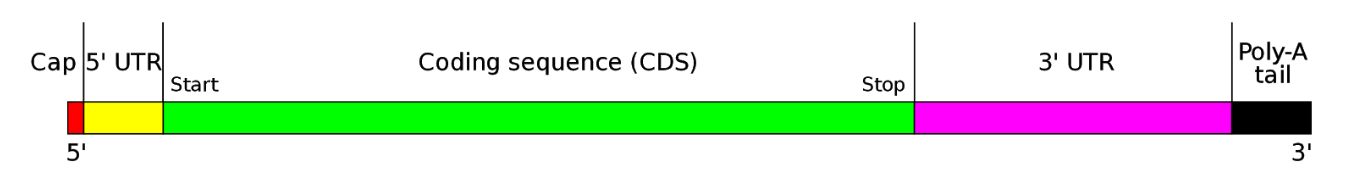
\includegraphics{C:/Users/lcqi/OneDrive/Desktop/1.png}

In cases like 5- the diseases are not rare so they can not be estimated.

\subsection{Problem 8}\label{problem-8}

\subsubsection{a.}\label{a.-3}

For London:

\begin{Shaded}
\begin{Highlighting}[]
\NormalTok{n11=}\DecValTok{911}
\NormalTok{n12=}\DecValTok{4578}
\NormalTok{n21=}\DecValTok{579}
\NormalTok{n22=}\DecValTok{4219}
\NormalTok{OR=n11}\OperatorTok{*}\NormalTok{n22}\OperatorTok{/}\NormalTok{(n12}\OperatorTok{*}\NormalTok{n21)}
\NormalTok{se=}\KeywordTok{sqrt}\NormalTok{(}\DecValTok{1}\OperatorTok{/}\NormalTok{n11}\OperatorTok{+}\DecValTok{1}\OperatorTok{/}\NormalTok{n12}\OperatorTok{+}\DecValTok{1}\OperatorTok{/}\NormalTok{n21}\OperatorTok{+}\DecValTok{1}\OperatorTok{/}\NormalTok{n22)}
\NormalTok{CI=}\KeywordTok{exp}\NormalTok{(}\KeywordTok{log}\NormalTok{(OR)}\OperatorTok{+}\KeywordTok{c}\NormalTok{(}\OperatorTok{-}\DecValTok{1}\NormalTok{,}\DecValTok{1}\NormalTok{)}\OperatorTok{*}\NormalTok{se}\OperatorTok{*}\KeywordTok{qnorm}\NormalTok{(}\FloatTok{0.975}\NormalTok{))}
\NormalTok{OR}
\end{Highlighting}
\end{Shaded}

\begin{verbatim}
## [1] 1.450019
\end{verbatim}

\begin{Shaded}
\begin{Highlighting}[]
\NormalTok{CI}
\end{Highlighting}
\end{Shaded}

\begin{verbatim}
## [1] 1.296051 1.622277
\end{verbatim}

For Manchester:

\begin{Shaded}
\begin{Highlighting}[]
\NormalTok{n11=}\DecValTok{361}
\NormalTok{n12=}\DecValTok{4532}
\NormalTok{n21=}\DecValTok{246}
\NormalTok{n22=}\DecValTok{3775}
\NormalTok{OR=n11}\OperatorTok{*}\NormalTok{n22}\OperatorTok{/}\NormalTok{(n12}\OperatorTok{*}\NormalTok{n21)}
\NormalTok{se=}\KeywordTok{sqrt}\NormalTok{(}\DecValTok{1}\OperatorTok{/}\NormalTok{n11}\OperatorTok{+}\DecValTok{1}\OperatorTok{/}\NormalTok{n12}\OperatorTok{+}\DecValTok{1}\OperatorTok{/}\NormalTok{n21}\OperatorTok{+}\DecValTok{1}\OperatorTok{/}\NormalTok{n22)}
\NormalTok{CI=}\KeywordTok{exp}\NormalTok{(}\KeywordTok{log}\NormalTok{(OR)}\OperatorTok{+}\KeywordTok{c}\NormalTok{(}\OperatorTok{-}\DecValTok{1}\NormalTok{,}\DecValTok{1}\NormalTok{)}\OperatorTok{*}\NormalTok{se}\OperatorTok{*}\KeywordTok{qnorm}\NormalTok{(}\FloatTok{0.975}\NormalTok{))}
\NormalTok{OR}
\end{Highlighting}
\end{Shaded}

\begin{verbatim}
## [1] 1.22236
\end{verbatim}

\begin{Shaded}
\begin{Highlighting}[]
\NormalTok{CI}
\end{Highlighting}
\end{Shaded}

\begin{verbatim}
## [1] 1.033641 1.445536
\end{verbatim}

For Newcastle:

\begin{Shaded}
\begin{Highlighting}[]
\NormalTok{n11=}\DecValTok{396}
\NormalTok{n12=}\DecValTok{6598}
\NormalTok{n21=}\DecValTok{219}
\NormalTok{n22=}\DecValTok{5261}
\NormalTok{OR=n11}\OperatorTok{*}\NormalTok{n22}\OperatorTok{/}\NormalTok{(n12}\OperatorTok{*}\NormalTok{n21)}
\NormalTok{se=}\KeywordTok{sqrt}\NormalTok{(}\DecValTok{1}\OperatorTok{/}\NormalTok{n11}\OperatorTok{+}\DecValTok{1}\OperatorTok{/}\NormalTok{n12}\OperatorTok{+}\DecValTok{1}\OperatorTok{/}\NormalTok{n21}\OperatorTok{+}\DecValTok{1}\OperatorTok{/}\NormalTok{n22)}
\NormalTok{CI=}\KeywordTok{exp}\NormalTok{(}\KeywordTok{log}\NormalTok{(OR)}\OperatorTok{+}\KeywordTok{c}\NormalTok{(}\OperatorTok{-}\DecValTok{1}\NormalTok{,}\DecValTok{1}\NormalTok{)}\OperatorTok{*}\NormalTok{se}\OperatorTok{*}\KeywordTok{qnorm}\NormalTok{(}\FloatTok{0.975}\NormalTok{))}
\NormalTok{OR}
\end{Highlighting}
\end{Shaded}

\begin{verbatim}
## [1] 1.441807
\end{verbatim}

\begin{Shaded}
\begin{Highlighting}[]
\NormalTok{CI}
\end{Highlighting}
\end{Shaded}

\begin{verbatim}
## [1] 1.217644 1.707237
\end{verbatim}

\subsubsection{b.}\label{b.-3}

We need the weights of different locations, wether disease and locations
are independent etc..

\subsection{Problem 9}\label{problem-9}

\begin{Shaded}
\begin{Highlighting}[]
\NormalTok{data=}\KeywordTok{matrix}\NormalTok{(}\KeywordTok{c}\NormalTok{(}\DecValTok{10}\NormalTok{,}\DecValTok{8}\NormalTok{,}\DecValTok{1}\NormalTok{,}\DecValTok{1}\NormalTok{),}\DecValTok{2}\NormalTok{)}
\KeywordTok{mcnemar.test}\NormalTok{(data,}\DataTypeTok{correct =} \OtherTok{FALSE}\NormalTok{)}
\end{Highlighting}
\end{Shaded}

\begin{verbatim}
## 
##  McNemar's Chi-squared test
## 
## data:  data
## McNemar's chi-squared = 5.4444, df = 1, p-value = 0.01963
\end{verbatim}

\subsection{Problem 10}\label{problem-10}

\begin{Shaded}
\begin{Highlighting}[]
\NormalTok{data=}\KeywordTok{matrix}\NormalTok{(}\KeywordTok{c}\NormalTok{(}\DecValTok{40}\NormalTok{,}\DecValTok{20}\NormalTok{,}\DecValTok{16}\NormalTok{,}\DecValTok{3}\NormalTok{),}\DecValTok{2}\NormalTok{)}
\KeywordTok{mcnemar.test}\NormalTok{(data,}\DataTypeTok{correct =}\NormalTok{ F)}
\end{Highlighting}
\end{Shaded}

\begin{verbatim}
## 
##  McNemar's Chi-squared test
## 
## data:  data
## McNemar's chi-squared = 0.44444, df = 1, p-value = 0.505
\end{verbatim}

\subsection{Problem 11}\label{problem-11}


\includegraphics{C:/Users/lcqi/OneDrive/Desktop/2.png}\\
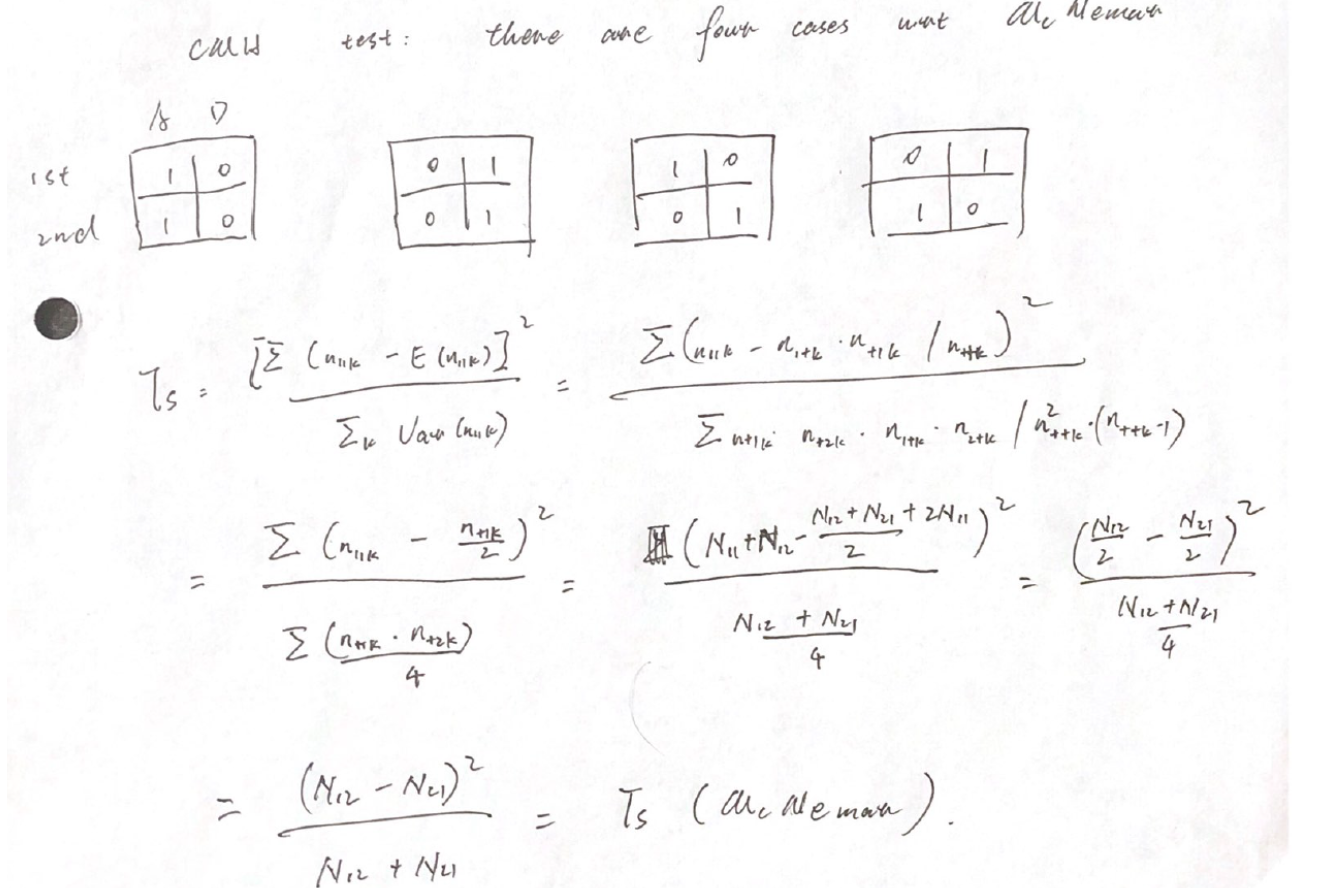
\includegraphics{C:/Users/lcqi/OneDrive/Desktop/0.png}

\subsection{Problem 12}\label{problem-12}

\subsubsection{a.}\label{a.-4}

\begin{longtable}[]{@{}llll@{}}
\toprule
& Northeast & Southeast & West\tabularnewline
\midrule
\endhead
Northeast & & n12(p12) & n13(p13)\tabularnewline
Southeast & n21(p21) & & n23(p23)\tabularnewline
West & n31(p31) & n32(p32) &\tabularnewline
\bottomrule
\end{longtable}

\(H_0 : p12=p21=p31=p13=p23=p32\)\\
\(H_A :\) at least two of p not equal to each other.

\subsubsection{b.}\label{b.-4}

Expected table :

\begin{longtable}[]{@{}llll@{}}
\toprule
& Northeast & Southeast & West\tabularnewline
\midrule
\endhead
Northeast & & 201 & 247.5\tabularnewline
Southeast & 201 & & 186.5\tabularnewline
West & 247.5 & 186.5 &\tabularnewline
\bottomrule
\end{longtable}

Observed table :

\begin{longtable}[]{@{}llll@{}}
\toprule
& Northeast & Southeast & West\tabularnewline
\midrule
\endhead
Northeast & & 267 & 255\tabularnewline
Southeast & 135 & & 139\tabularnewline
West & 240 & 234 &\tabularnewline
\bottomrule
\end{longtable}

\subsubsection{c.}\label{c.}

TS = 67.99

\begin{Shaded}
\begin{Highlighting}[]
\KeywordTok{pchisq}\NormalTok{(}\FloatTok{67.99}\NormalTok{,}\DecValTok{3}\NormalTok{,}\DataTypeTok{lower.tail =}\NormalTok{ F)}
\end{Highlighting}
\end{Shaded}

\begin{verbatim}
## [1] 1.149672e-14
\end{verbatim}

The probabilities of moving between different places are not symmetric.


\end{document}
